\documentclass[12pt, a4paper]{article}
\usepackage{../notesheets}
\usepackage{epsdice}
\usepackage{tikz}
\usetikzlibrary{shapes.geometric, arrows}

\newcommand{\Var}{\operatorname{Var}}
%%%%%%%%%%%%%%%%%%%%%%%%%%%%%%%%%%%%%%%%%%%%%%%%%%
\author{Math 1220}
\title{Notesheet. Section 11.4 Part 2: Series with Positive Terms} 
\date{}

\begin{document}
\maketitle
\nameline
%%%%%%%%%%%%%%%%%%%%%%%%%%%%%%%%%%%%%%%%%%%%%%%%%%
\begin{ex}
Determine the convergence of the following series:
\begin{enumerate}
\item \(\sum_{n=1}^\infty \frac{5n-1}{2n^3+4n+3}\)
  \vspace{1.5in}
\item \(\sum_{n=1}^\infty \frac{9+\sin(n)}{n^3}\)
\end{enumerate}
\end{ex}
Other series to try at home:\\

\(\sum_{n=1}^\infty \frac{9+\sin(n)}{n}, \sum_{n=2}^\infty
\frac{\pi^n}{e^n-1}, \sum_{n=2}^\infty \frac{1}{2\sqrt{n^2-1}},
\sum_{n=1}^\infty \frac{1}{n^n}\) (Hint: \(n^n \geq n^2\)).
\begin{ex}
  True or False?
  \begin{enumerate}
  \item We can apply the comparison test on \(\sum_{n=1}^\infty
    \frac{(-1)^n}{n^2}\)
    \vspace{1in}
  \item If \(\sum a_n, \sum b_n, \) and \(\sum c_n\) are all series
    with positive terms, \(\sum a_n\) is convergent, and \(b_n+c_n
    \leq a_n\) for all \(n\), then \(\sum b_n\) and \(\sum c_n\) are
    convergent.
    \vspace{1in}
  \item If \(\sum a_n, \sum b_n, \) and \(\sum c_n\) are all series
    with positive terms, \(\sum a_n\) is divergent and \(b_n + c_n
    \geq a_n\) for 
    all \(n\), then \(\sum b_n\) and \(\sum c_n\) are divergent.
  \end{enumerate}
\end{ex}
\begin{rmk}
  A heuristic approach to solving series convergence problems in this
  class goes as follows \\
  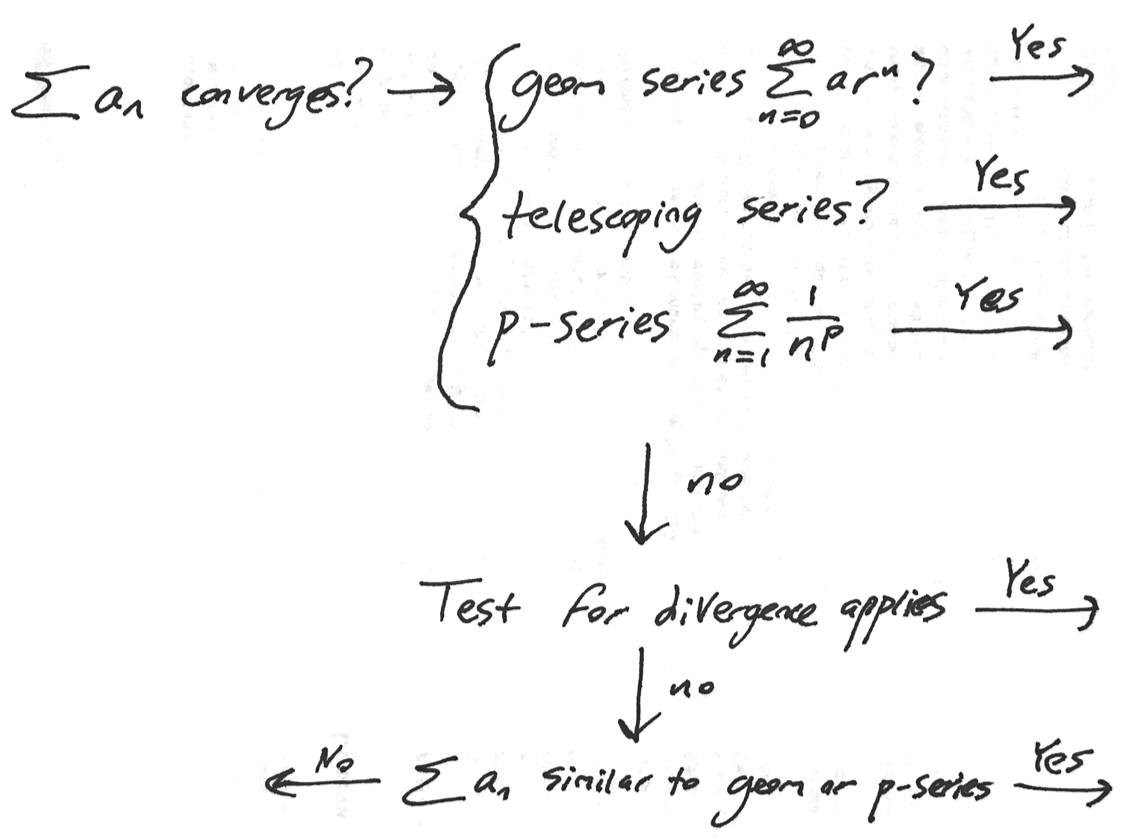
\includegraphics[scale=0.35]{images/incomplete-series-convergence-flowchart}
\end{rmk}
%%%%%%%%%%%%%%%%%%%%%%%%%%%%%%%%%%%%%%%%%%%%%%%%%% 
\end{document}
